\chapter{Өргөтгөсөн тодорхой интеграл}

Тодорхой интегралын дээд эсвэл доод хил нь $\infty$ (эсвэл $-\infty$) байх, эсвэл 
интегралчлах функц нь интегралчлах мужын зарим цэг дээр тасралттай байх 
тохиолдолд интегралыг нийлбэрийн хязгаараар тодорхойлох боломжгүй юм. 
Ийм интегралуудыг бодох шаардлага гардаг тул эдгээр интегралыг хязгаар ашиглан тодорхойлдог.

\section{Зааглагдаагүй мужаар авсан интеграл}

\begin{definition}[I төрлийн өргөтгөсөн интеграл]
$f$ функц нь $[a,+\infty)$ дээр тодорхой байг. Хэрэв
\[
\lim_{t\to\infty}\int_a^{t} f(x)\,dx
\]
хязгаар оршин байвал түүнийг $f(x)$ функцээс $[a,\infty)$ завсараар авсан тодорхой интеграл гэнэ.  

\[
\int_a^{\infty} f(x)\,dx := \lim_{t\to\infty}\int_a^{t}f(x)\,dx.
\]

Хэрэв хязгаар төгсгөлөг утгатай байвал интегралыг \textbf{нийлдэг}, бусад үед \textbf{сарнидаг интеграл} гэнэ.
\end{definition}

Доод хил эсвэл хоёр хил нь зааглагдаагүй үед адилаар тодорхойлно.

\[
\int_{-\infty}^{b} f(x)\,dx := \lim_{t\to -\infty}\int_t^{b}f(x)\,dx,
\qquad
\int_{-\infty}^{\infty} f(x)\,dx := 
\int_{-\infty}^{c} f(x)\,dx + \int_{c}^{\infty} f(x)\,dx.
\]

\begin{example}\label{x^{-2}}
$y=\dfrac{1}{x^2}$ ($x\ge1$) графикийн доорх талбайг олъё:
\[
\int_{1}^{\infty} \frac{dx}{x^2}
= \lim_{t\to\infty}\int_{1}^{t} x^{-2}\,dx
= \lim_{t\to\infty}\left[-x^{-1}\right]_{1}^{t}
= \lim_{t\to\infty}\left( -\frac{1}{t} + 1\right)
= 1.
\]
Иймээс
\[
\int_{1}^{\infty}\frac{dx}{x^2} = 1 \quad (\text{нийлнэ}).
\]
\end{example}

\section{Үл зааглагдах функцийн интеграл}

\begin{definition}[II төрлийн өргөтгөсөн интеграл]
$f$ функц нь $(a,b)$ дээр тасралтгүй тодорхойлогдсон боловч $x=a$ дээр төгсгөлгүй тасралттай байг.  
Хэрэв
\[
\lim_{t\to a+}\int_{t}^{b} f(x)\,dx
\]
хязгаар оршин байвал түүнийг $y=f(x)$ функцээс $(a,b)$ завсараар авсан тодорхой интеграл гэнэ.
\[
\int_{a}^{b} f(x)\,dx := \lim_{t\to a+}\int_{t}^{b}f(x)\,dx.
\]
Хэрэв $x=b$ дээр төгсгөлгүй тасралттай бол
\[
\int_a^{b}f(x)\,dx = \lim_{t\to b-}\int_{a}^{t} f(x)\,dx.
\]
Хэрэв хязгаар төгсгөлөг байвал интегралыг \textbf{нийлдэг}, үгүй бол \textbf{сарнидаг интеграл} гэнэ.
\end{definition}

\begin{example}\label{x^{-1/2}}
$f(x) = \dfrac{1}{\sqrt{x}}$ нь $(0,1)$ дээр тодорхойлогдох боловч $x\to 0^{+}$ үед $f(x)\to\infty$.
Иймд 
\[
\int_{0}^{1}\frac{dx}{\sqrt{x}}
= \lim_{t\to0+}\int_{t}^{1} x^{-1/2}\,dx
= \lim_{t\to0+}\left[2\sqrt{x}\right]_{t}^{1}
= \lim_{t\to0+}(2 - 2\sqrt{t})
= 2.
\]
Иймээс интеграл \textbf{нийлнэ}.
\end{example}

\begin{example}\label{x^-1}
\[
\int_{0}^{1}\frac{dx}{x}
= \lim_{t\to0+}\int_{t}^{1} \frac{dx}{x}
= \lim_{t\to0+} [\ln x]_{t}^{1}
= \lim_{t\to0+}(0 - \ln t)
= +\infty.
\]
Иймээс интеграл \textbf{сарнина}.
\end{example}

\section{Нийлэлт, сарнилтыг тодорхойлох шинжүүр}

\begin{theorem}Жиших шинжүүр]
$x\ge a$ үед $0\le f(x)\le g(x)$ байг.

\begin{enumerate}
\item Хэрэв $\displaystyle\int_{a}^{\infty} g(x)\,dx$ нийлбэл  
\quad $\displaystyle\int_{a}^{\infty} f(x)\,dx$ мөн нийлнэ.
\item Хэрэв $\displaystyle\int_{a}^{\infty} f(x)\,dx$ сарнивал  
\quad $\displaystyle\int_{a}^{\infty} g(x)\,dx$ мөн сарнина.
\end{enumerate}
\end{theorem}
Харьцуулах шинжүүр хэрэглэхийн тулд өгсөн интегралтай төстэй нийлэх сарнихыг нь мэддэг интеграл авч үзэх хэрэгтэй. Ийм зорилгоор ихэвчлэн $f(x)=x^{-p}$ функцийн интегралыг авч үздэг.
\begin{example}[ $x^{-p}$ функцийн интеграл]
 Жишээ \ref{x^{-2}} харахад $\displaystyle\int\limits_1^{\infty}x^{-p}dx$ интеграл $p=2$ үед нийлж байна. Ерөнхий тохиолдолд дараах нөхцөл биелнэ.
 \[
\int_{1}^{\infty} \frac{dx}{x^{p}}
\quad\text{нийлэх } \Longleftrightarrow\; p>1.
\]
Тодруулбал,
\[
\int_{1}^{\infty} x^{-p}\,dx =
\begin{cases}
\displaystyle \frac{1}{p-1}, & p>1,\\[4pt]
+\infty, & p\le1.
\end{cases}
\] байна. \\
Мөн Жишээ \ref{x^{-1/2}} ба  \ref{x^-1}  харахад $\displaystyle\int\limits_1^{\infty}x^{-p} dx$ интеграл $p= 1/2$ үед нийлж, $p=1$ үед сарниж байна. Ерөнхий тохиолдолд дараах нөхцөл биелнэ.
 \[
\int_{0}^{1} x^{-p}\,dx
\quad\text{нийлэх } \Longleftrightarrow\; p<1.
\]

Тодруулбал,
\[
\int_{0}^{1} x^{-p}\,dx =
\begin{cases}
\displaystyle \frac{1}{1-p}, & p<1,\\[4pt]
+\infty, & p\ge1.
\end{cases}
\]
\end{example}

\begin{example}[Жиших шинжүүр хэрэглэх]
Дараах интеграл нийлэх эсэхийгтодорхойлоё.
\[
\int_{1}^{\infty} \frac{dx}{1+x^{3}}.
\]

Их $x$ үед $1+x^3\sim x^{3}$.
\[
0 < \frac{1}{1+x^{3}} \le \frac{1}{x^{3}}, \qquad x\ge1.
\]
жиших шинжүүрээр $p=3>1$ тул  
\[
\int_{1}^{\infty}\frac{dx}{x^{3}}
\text{ нийлэх тул}
\quad\Rightarrow\quad
\int_{1}^{\infty}\frac{dx}{1+x^{3}}
\text{ мөн нийлнэ.}
\]
\end{example}
\section{Тодорхой интегралын хэрэглээ}
\subsection{Хоёр муруйн хоорондох талбай}
$y=f(x) , \, y=g(x)$ функцүүдийн графикуудын хоорондох хашигдсан $x=a , \, x=b$ хэсгийн талбайг
\[
A=\int_{a}^{b} |f(x)-g(x)|\,dx.
\]
томьёогоор олно.
\begin{example} $y=2x$, $y=x^2$ муруйн хоорондох талбай ол.\\
\begin{minipage}{0.6\textwidth}
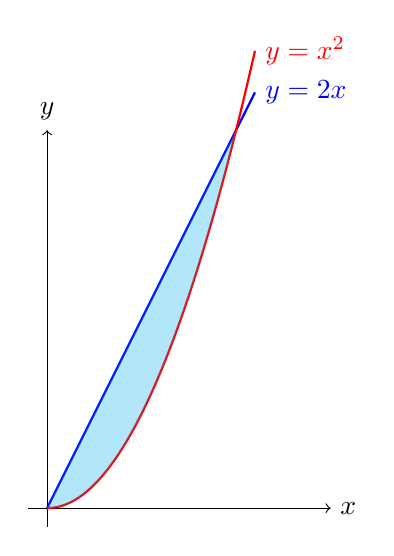
\begin{tikzpicture}[scale=1.2]
\draw[->] (-0.2,0) -- (3,0) node[right] {$x$};
\draw[->] (0,-0.2) -- (0,4) node[above] {$y$};

\draw[domain=0:2.2, smooth, variable=\x, blue, thick]
  plot ({\x},{2*\x}) node[right] {$y=2x$};

\draw[domain=0:2.2, smooth, variable=\x, red, thick]
  plot ({\x},{\x*\x}) node[right] {$y=x^2$};

\begin{scope}
\clip (0,0) --
  plot[domain=0:2] ({\x},{2*\x}) --
  plot[domain=2:0] ({\x},{\x*\x}) -- cycle;

\fill[cyan, opacity=.3] (0,0) rectangle (3,4);
\end{scope}
\end{tikzpicture}  
\end{minipage}
\begin{minipage}{0.4\textwidth}
   $y=2x$, $y=x^2$ муруйн хоорондох талбайг олохын тулд тэдгээрийн огтлолцлын цэгүүдийг олох хэрэгтэй. $2x=x^2$ тэгшитгэл бодвол $x=0,\, x=2$ шийдүүд гарна. Иймд олох талбай нь 
\[
A=\int_{0}^{2} |2x-x^2|\,dx=\int_{0}^{2} (2x-x^2)\,dx=\frac{4}{3}.
\] болно. 
\end{minipage}
\end{example}
\begin{example}
    $f(x)=\cos x$, $g(x)=\sin x$, $[\pi/6,\pi/4]$ интервал дээрх талбай ол.\\
Харгалзах график зурж харвал:

\begin{center}
\begin{tikzpicture}[scale=2]
% Axes
\draw[->] (-0.2,0)--(1.2,0) node[right]{$x$};
\draw[->] (0,-0.2)--(0,1.2) node[above]{$y$};

% Functions
\draw[domain=0:0.9,samples=100,thick,blue]
  plot(\x,{cos(\x r)}) node[right]{$y=\cos x$};

\draw[domain=0:0.9,samples=100,thick,red]
  plot(\x,{sin(\x r)}) node[right]{$y=\sin x$};

% Fill area
\fill[green!60,opacity=0.7]
  plot[domain=0.5:0.785] (\x,{cos(\x r)})
  -- plot[domain=0.785:0.5] (\x,{sin(\x r)})
  -- cycle;
\draw[dashed] (0.785,0)--(0.785,0.71);
\draw[dashed] (0.5,0)--(0.5,0.855);
\node at (0.785,-0.2) {$\tfrac{\pi}{4}$};
\node at (0.5,-0.2){$\tfrac{\pi}{6}$};
\end{tikzpicture}
\end{center}
$f(x)=\cos x$, $g(x)=\sin x$ функцүүдийн хувьд
$[0,\pi/4]$ интервал дээр $y=\cos x$ функцийн график дээгүүр нь байгаа тул 
\[
\text{Талбай=}\int_{\pi/6} ^{\pi/4}|\cos x-\sin x|\,dx
=\int_{\pi/6} ^{\pi/4} (\cos x-\sin x)\,dx
=
\Bigl[\sin x+\cos x\Bigr]_{\pi/6}^{\pi/4}
=\sqrt2-1.
\]

\end{example}
\section{Биетийн эзлэхүүн олох}
\subsection{Хөндлөн огтлолын арга (эргэлтийн биш биет)}

Хэрэв биетийн хөндлөн огтлолын талбай нь $A(x)$ бол:
\[
V = \int_{a}^{b} A(x)\,dx.
\]

\subsection*{Жишээ}
$A(x)=x^2$ байвал ($0\le x\le 3$):
\[
V=\int_{0}^{3} x^2 dx = 9.
\]
\begin{center}
\begin{tikzpicture}[scale=1.1]

% Axes
\draw[->] (-0.5,0) -- (4.5,0) node[right] {$x$};
\draw[->] (0,-0.5) -- (0,4.5) node[above] {$y$};

% Parabola y = x^2
\draw[thick,blue,domain=0:2,samples=100]
  plot(\x,{(\x)^2}) node[right] {$y=x^2$};

% Shaded region under curve
\fill[blue!20,opacity=0.5]
  (0,0) --
  plot[domain=0:2] (\x,{(\x)^2}) --
  (2,0) -- cycle;

% Sample disk at x = x0
\def\xo{1.3}
\pgfmathsetmacro{\yo}{(\xo)*(\xo)}

% Radius
\draw[red,thick] (\xo,0) -- (\xo,\yo)  node[midway,right] {$r=x^2$};

% Disk (ellipse to show rotation)
\draw[red,thick] (\xo,\yo) ellipse (0.35 and 0.12);

% Axis of rotation
\draw[dashed] (-0.3,0) -- (4.3,0);
\node at (3.8,-0.25) {$x$-тэнхлэг};

% Labels
\node at (2.6,3.5) {Эргэх биет};
\node at (1.35,-0.3) {$x$};

\end{tikzpicture}
\end{center}

\begin{center}
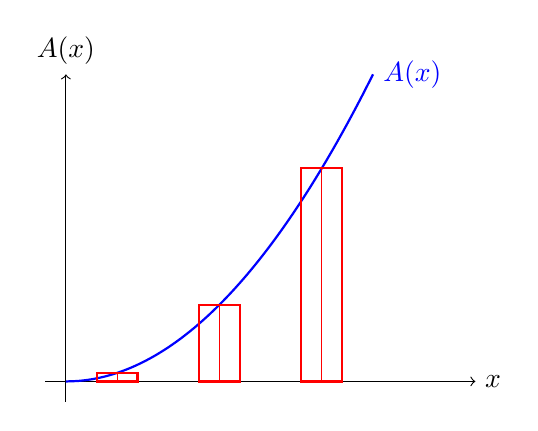
\begin{tikzpicture}[scale=1.3]
\draw[->] (-0.2,0) -- (4,0) node[right] {$x$};
\draw[->] (0,-0.2) -- (0,3) node[above] {$A(x)$};

\draw[domain=0:3, smooth, variable=\x, blue, thick]
  plot ({\x},{(\x)^2/3}) node[right] {$A(x)$};

\foreach \x in {0.5,1.5,2.5}{
  \draw[red] (\x,0) -- (\x,{(\x)^2/3});
  \draw[red, thick] (\x-0.2,0) rectangle (\x+0.2,{(\x)^2/3});
}
\end{tikzpicture}
\end{center}

%%%%%%%%%%%%%%%%%%%%%%%%%%%%%%%%%%%%%%%%%%%%%%%%%%%%%%
\section{Эргүүлж үүсгэсэн биет}

\subsection{Дискний арга}
\[
V=\pi\int_{a}^{b} f(x)^2\,dx.
\]

\subsection{Бүрхүүл (shell) арга}
\[
V = 2\pi\int_{a}^{b} x f(x)\,dx.
\]

\subsection*{Жишээ}
$y=\sqrt{x}$ муруйг $y$-тэнхлэгийн эргэн эргүүлэх ($0\le x\le4$):
\[
V=2\pi\int_{0}^{4} x\sqrt{x} dx = \frac{128\pi}{5}.
\]

\subsection*{TikZ зураг}

\begin{center}
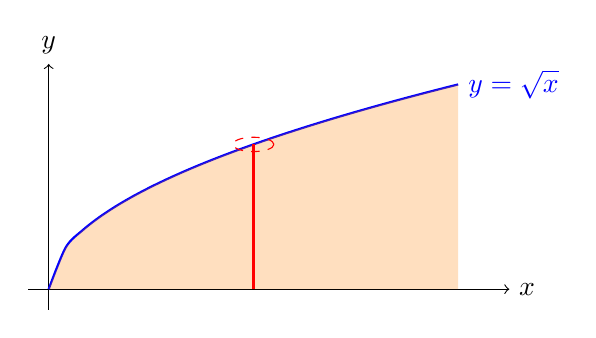
\begin{tikzpicture}[scale=1.3]

\draw[->] (-0.2,0)--(4.5,0) node[right] {$x$};
\draw[->] (0,-0.2)--(0,2.2) node[above] {$y$};

\draw[domain=0:4, smooth, variable=\x, blue, thick]
  plot({\x},{sqrt(\x)}) node[right] {$y=\sqrt{x}$};

\fill[orange, opacity=.25] (0,0)--plot[domain=0:4]({\x},{sqrt(\x)})--(4,0)--cycle;

\draw[red, thick] (2,0)--(2,{sqrt(2)});
\draw[red, dashed] (2,{sqrt(2)}) circle (0.2 and 0.07);

\end{tikzpicture}
\end{center}

%%%%%%%%%%%%%%%%%%%%%%%%%%%%%%%%%%%%%%%%%%%%%%%%%%%%%%
\section{Нэмэлт жишээ — 2 муруйн хоорондох талбай}

$f(x)=\cos x$, $g(x)=\sin x$, $[0,\pi/4]$ интервал дахь талбай:

\[
A=\int_{0}^{\pi/4} (\cos x - \sin x)\, dx.
\]

%%%%%%%%%%%%%%%%%%%%%%%%%%%%%%%%%%%%%%%%%%%%%%%%%%%%%%
\section{Семинар}
\begin{enumerate}
    \item $y=x^2$ ба $y=x+3$ функцийн графикуудаар хүрээлэгдсэн хэсгийн талбайг ол.
    \item $y=\dfrac{1}{1+x^2}$ , $(1;+\infty)$  хэсгийн доорх талбайг ол.
    \item $y=f(x)$ функцийн гарфикийн $(a;b)$ хэсгийг $ox$ тэнхлэгийг тойруулан эргүүлэхэд үүсэх биетийн эзэлхүүн $\displaystyle\pi\int\limits_a^b f^2(x) dx$ байхыг батал.
    \item $y=\sqrt{x}$  функцийн гарфикийн $(1;3)$ хэсгийг $ox$ тэнхлэгийг тойруулан эргүүлэхэд үүсэх биетийн эзэлхүүн ол.
    \item Интеграл бод. 
    \begin{enumerate}
        \item $\displaystyle\int\limits_1^5\dfrac{1}{x\sqrt{x-1}} dx$
        \item $\displaystyle\int\limits_5^{\infty}\dfrac{1}{x\sqrt{x-1}}$
        \item $\displaystyle\int\limits_{-\infty}^1\dfrac{1}{(1+x^2)^2}$
        \item $\displaystyle\int\limits_0^{\infty}x^3e^{-x^2}dx$
    \end{enumerate}
    \item Талбай ол.
    \begin{enumerate}
        \item $y=\sin x\quad , 0\leq x\leq \pi$
        \item $y=\ln x \quad , 1\leq x\leq e$
        \item $y=e^x$ ба $y=3x+1$ хүрээлэгдсэн
        \item $y=x(x-1)(x-2)$ ба $ox$ тэнхлэгээр хүрээлэгдсэн
    \end{enumerate}
    \item  Муруйн урт ол.
    \begin{enumerate}
        \item $y=\ln x\quad , \sqrt{3}\leq x\leq \sqrt{5}$
        \item $y=\dfrac{x^2}{2}-\ln x \quad , 1\leq x\leq e$
    \end{enumerate}
     \item  Эзэлхүүн ол.
    \begin{enumerate}
        \item $y=\cos x$ функцийн $ 0\leq x\leq \dfrac{\pi}{2}$ хэсгийг $ox$ тэнхлэгийг тойруулан эргүүлэхэд үүсэх биет
        \item 
        $R=1$ , $H=2$ үед эдэлхүүн ол\\
        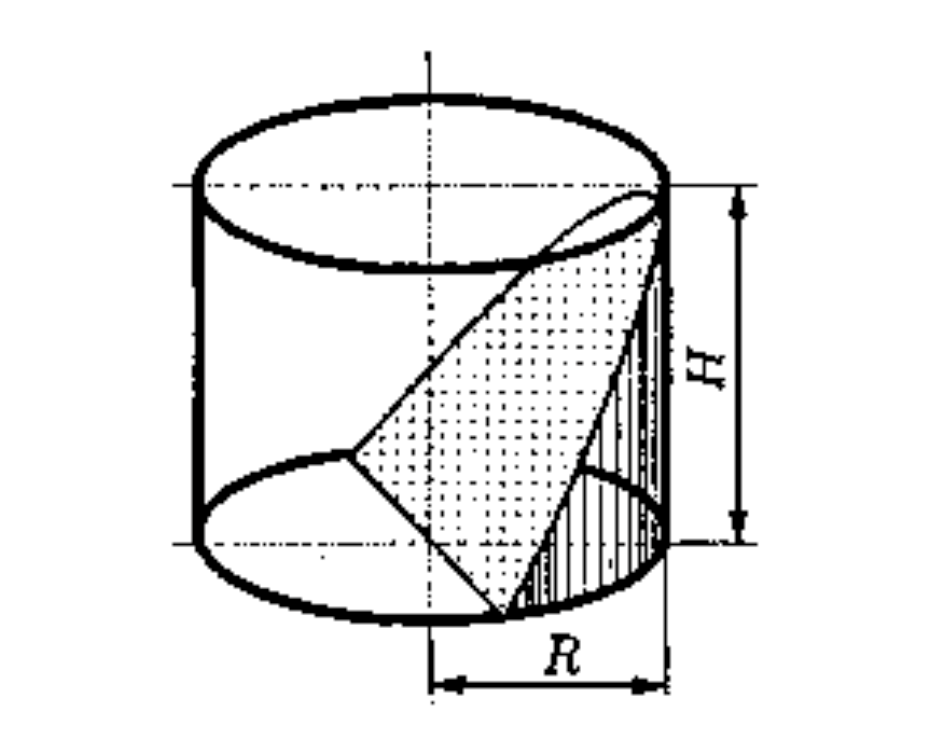
\includegraphics[scale=0.3]{pictures/cyltairdas.png}
        \item $h$ өндөртэй, $r$ ба $R$ суурийн радиустай огтлогдсон конусын эзэлхүүн бодох томьёог эргэлтийн биеийн эзэлхүүн олох томьёог ашиглан гарга. $r=R=2$ үед бодож шалга.
    \end{enumerate}
\end{enumerate}